\graphicspath{ {./images/1_electrostatic/} }

\chapter{Electrostática}

La teoría electromagnética clásica estudia los fenómenos eléctricos y magnéticos, describiendo sus características y las leyes que los gobiernan.  

Cuando se habla de teoría clásica, se hace referencia a que se basa en la mecánica clásica de Isaac Newton. En esta mecánica se utilizan conceptos como partículas, trayectorias y las leyes del movimiento de Newton. De manera similar, en la teoría electromagnética se aplican estos conceptos a las cargas eléctricas y a los campos eléctricos y magnéticos. Es decir, en lugar de hablar solo de partículas y fuerzas mecánicas, hablaremos de partículas cargadas, fuerzas eléctricas y campos electromagnéticos. 

El electromagnetismo es una teoría de campos. Por ejemplo, una carga eléctrica genera un campo eléctrico a su alrededor, mientras que un imán produce un campo magnético en el espacio que lo rodea. Estos campos son perturbaciones en el espacio que afectan a otras cargas o imanes cercanos y pueden describirse matemáticamente. 

A lo largo de la historia, se ha comprobado que existen dos tipos de carga eléctrica: positiva y negativa. Las cargas del mismo tipo se repelen, mientras que las de signos opuestos se atraen.

\section{Carga y Materia}

Todo lo que nos rodea, como una pelota, el aire, una planta o nuestro propio cuerpo, está formado por átomos. Los átomos, a su vez, están compuestos por tres tipos de partículas: protones, neutrones y electrones. Los protones y neutrones se encuentran en el núcleo del átomo, mientras que los electrones se mueven alrededor en la corteza. Los protones tienen carga positiva, los electrones carga negativa, y los neutrones no tienen carga. 

Esta estructura corresponde a un modelo atómico, que es una representación que nos ayuda a entender cómo está compuesto un átomo y cómo se comporta. A lo largo del tiempo han existido distintos modelos atómicos, pero uno de los más conocidos es el modelo de Bohr. Según este modelo, los electrones giran alrededor del núcleo en órbitas circulares, cada una con un nivel de energía específico. Cuando un electrón cambia de órbita, absorbe o emite energía en forma de luz. La figura \ref{fig_modelo_atomico} muestra una representación del átomo de Helio.

La carga elemental \(e\) es la cantidad más pequeña de carga eléctrica libre que se conoce en la naturaleza. Es la carga que poseen los protones y electrones, pero con signo opuesto:
\begin{itemize}
  \item Electrón: \( -e = -\qty{1.602e-19}{\coulomb}\)
  \item Protón: \( +e = \qty{1.602e-19}{\coulomb} \)
\end{itemize}
\begin{marginfigure}
  \centering
  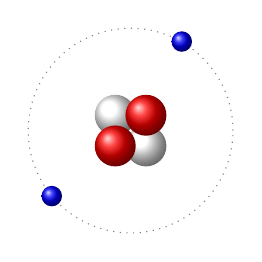
\begin{tikzpicture}[scale=1.3]
    \shade[ball color=white] (-.15,.15) circle (.2);
    \shade[ball color=white] (.15,-.15) circle (.2);
    \shade[ball color=red] (-.15,-.15) circle (.2);
    \shade[ball color=red] (.15,.15) circle (.2);
    \draw[dotted,gray] (0,0) circle (1);
    \shade[ball color=blue] (.5,.87) circle (.1);
    \shade[ball color=blue] (-.77,-.64) circle (.1);
  \end{tikzpicture}
  \caption{Representación del modelo básico de un átomo.}
  \label{fig_modelo_atomico}
\end{marginfigure}

La carga elemental es fundamental porque todas las cargas eléctricas observadas en la naturaleza son múltiplos enteros de \( e \). Es decir, cualquier carga presente en un objeto es el resultado de un exceso o déficit de electrones. Este principio se conoce como la ley de conservación de la carga eléctrica, y establece que la carga eléctrica no se crea ni se destruye, solo se transfiere de un cuerpo a otro. Un objeto es eléctricamente neutro cuando tiene igual número de ambos. Si un objeto adquiere carga negativa, significa que ha ganado electrones, y si adquiere carga positiva, significa que ha perdido electrones. Cuando un objeto se carga, no se están creando nuevas cargas, sino que se están moviendo electrones de un cuerpo a otro. Por ejemplo: en la electrización por frotamiento, un material transfiere electrones a otro, dejando uno cargado positivamente y el otro negativamente.

Denominaremos con la letra \( Q \) o \( q \) a la carga eléctrica de un objeto. La carga se mide en Coulombs (\unit{\coulomb}). Un Coulomb es una cantidad de carga muy grande, por lo que en la práctica se utilizan submúltiplos como el milicoulomb (\unit{\milli\coulomb}) o el microcoulomb (\unit{\micro\coulomb}).


% \subsection{Fuerza eléctrica}

\subsubsection{Ley de Coulomb}

La electrostática estudia las cargas eléctricas en \hl{\textbf{reposo}}. La ley de Coulomb establece que \textbf{la fuerza entre dos cargas puntuales} es:
\begin{equation}
    F = k_e \frac{\abs{q_1} \cdot \abs{q_2}}{r^2}
    \label{eq:ley_coulomb}
\end{equation}
donde:
\begin{itemize}
    \item \( k_e \) es la constante de Coulomb: \( 8.9876 \times 10^9 \, \frac{\si{\newton\meter\squared}}{\si{\coulomb\squared}} \).
    \begin{itemize}
        \item \( k_e \) se obtiene de  \( \frac{1}{4\pi\epsilon_0} \) y,
        \item \( \epsilon_0 \) es la permitividad del vacío: \( 8.85 \times 10^{-12} \,\frac{\si{\coulomb\squared}}{\si{\newton\meter\squared}} \)
    \end{itemize}
    \item \( q_1 \) y \( q_2 \) son las cargas.
    \item \( r \) es la distancia entre las cargas.
\end{itemize}

Es muy importante notar que la \textbf{Ley de Coulomb} \eqref{eq:ley_coulomb} se aplica estrictamente a \hl{cargas puntuales}, es decir, cargas que se consideran concentradas en un solo punto sin dimensiones espaciales. En la ecuación anterior \eqref{eq:ley_coulomb}, se obtiene la magnitud de la fuerza eléctrica. La expresión vectorial de la fuerza eléctrica es:

\begin{equation}
    \vec{F}_e = k_e \frac{|q_1 q_2|}{r^2} \hat{r}
    \label{eq:ley_coulomb_vectorial}
\end{equation}
donde:
\begin{itemize}
    \item \( \vec{F}_e \) es el vector fuerza eléctrica entre dos cargas puntuales \( q_1 \) y \( q_2 \)
    \item \( \hat{r} \) es el vector unitario en la dirección que une ambas cargas.
\end{itemize}

Esto es importante tenerlo en cuenta ya que si se quiere saber la fuerza total sobre una carga \( q \) debido a varias cargas, se debe sumar vectorialmente las fuerzas individuales. La fuerza total sobre una carga \( q \) debido a un conjunto de cargas \( Q_i \) es:

\begin{equation}
    \vec{F} = \sum_i k \frac{|q \cdot Q_i|}{r_i^2} \hat{\mathbf{r_i}}
    \label{eq:ley_coulomb_vectorial_suma}
\end{equation}

\subsubsection{Cargas eléctricas}

La \textbf{carga eléctrica} es una propiedad fundamental de la materia que determina la interacción electromagnética entre partículas. Se trata de una magnitud escalar que puede ser de dos tipos: \textbf{positiva} o \textbf{negativa}. Las partículas con carga del mismo signo se repelen, mientras que las de signo opuesto se atraen.

La unidad de carga eléctrica en el \textbf{Sistema Internacional (SI)} es el \textbf{coulomb (\( \si{\coulomb} \))}. La carga elemental está representada por la carga del electrón (\( -e = -1.602 \times 10^{-19} \si{\coulomb} \)) y la del protón (\( e = +1.602 \times 10^{-19} \si{\coulomb} \)).

\begin{center}
    \setlength{\arrayrulewidth}{1pt}  % Grosor de líneas
    \renewcommand{\arraystretch}{1.3} % Espaciado vertical
    \arrayrulecolor{gray} % Color de líneas

    \begin{tabular}{ c c c }
        \hline
        \rowcolor{asparagus!30}
        \textbf{Partícula}  & \textbf{Carga (\si{\coulomb})}           & \textbf{Masa (\si{\kg})}   \\ \hline
        Electrón (e)        & \(-e = -1.602 \times 10^{-19}\)   & \(9.109 \times 10^{-31}\) \\
        Protón (p)          & \(+e = +1.602 \times 10^{-19}\)   & \(1.672 \times 10^{-27}\) \\
        Neutrón (n)         & \(0\)                             & \(1.675 \times 10^{-27}\) \\ \hline
    \end{tabular}
\end{center}

% \subsection{Campo eléctrico}

Para entender la definición del campo eléctrico desde el principio, debemos pensar en cómo se conceptualiza la interacción entre cargas eléctricas y en la necesidad de definir una propiedad del espacio que describa esta interacción.

Sabemos que las cargas eléctricas ejercen fuerzas unas sobre otras. Experimentalmente, se observa que cargas del mismo signo se repelen y cargas de signo opuesto se atraen. Esta interacción fue formulada matemáticamente por la Ley de Coulomb \eqref{eq:ley_coulomb_vectorial}, sin embargo, esta ley solo nos dice cómo una carga afecta a otra en particular, \hl{pero no describe una propiedad del espacio en sí}. Aquí es donde se introduce el concepto de \textbf{campo eléctrico}.

\begin{figure}[ht]
  \centering
  \includegraphics[width=0.6\textwidth]{field_concept.jpg}
  \caption{Se visualiza la perturbación el espacio al generar un campo eléctrico como movimiento de cargas.}
  \label{fig:concepto_campo_electrico}
\end{figure}

En lugar de pensar que una carga actúa instantáneamente sobre otra, se puede imaginar que una carga genera algo en el espacio a su alrededor que luego interactúa con otras cargas. Este ``algo'' es el \textbf{campo eléctrico}. La idea es la siguiente:

\begin{enumerate}
  \item Una carga fuente \( Q \) modifica el espacio circundante.
  \item Cualquier otra carga \( q \) que se coloque en ese espacio experimentará una fuerza debido a esta modificación.
  \item Para cuantificar esa modificación, definimos el campo eléctrico como la \textbf{fuerza por unidad de carga de prueba}.
\end{enumerate}

\subsubsection{Idea conceptual del campo eléctrico}

Si te preguntas qué es el campo eléctrico, puedes responder según la descripción previa: ``el campo eléctrico es una propiedad del espacio que rodea a una carga eléctrica capaz de interactuar con otras cargas''. Sin embargo la idea es entender qué significa que una carga eléctrica modifique las propiedades del espacio que la rodea. Veamos un ejemplo de esto para entenderlo mejor.

Supongamos que tengo una carga positiva (un protón) y quiero que se quede totalmente quieto. Entonces ¿Cómo podemos lograr esto? 
Bueno, pues es bastante sencillo. Buscamos alguna carga \( Q \) que a una distancia \( r \) haga que la carga \( q \) del protón anule las fuerzas que interactúan con la carga.

Supongamos que la única fuerza que está interactuando con el protón es la fuerza peso. Entonces tendríamos que encontrar cualquier combinación de \( Q \) y \( r \) que cumpla:

\[
  F_g = F_e \rightarrow m_p\, g - k_e \frac{Q \cdot q}{r^2} = 0
\]

Como nuestras incógnitas son \( Q \) y \( r \) vamos a tener infinitas posibilidades que solucionan muestro problema. Pero antes de dar por terminado el problema te pregunto ¿Qué tienen en común todas las soluciones?

Todas las soluciones están ocasionando el mismo efecto en el protón, una fuerza vertical y hacia arriba (en sentido opuesto al peso). Podríamos expresar esto diciendo: ``todas las soluciones generan una perturbación idéntica en el punto del espacio donde se encuentra el protón''. O, en otras palabras, todas las soluciones generan un campo eléctrico de las mismas características en donde está el protón.

Es más, cualquier partícula que coloquemos en el lugar del protón, con cualquier carga, por ejemplo una partícula con tres veces la carga del protón pero negativa, sentirá una fuerza proporcional a la que sentía el protón. En el caso de este ejemplo sería una fuerza igual a tres veces el peso del protón en el mimo sentido al peso (por ser negativa).

Para el ejemplo que vimos, el protón fué lo que llamaremos \textit{carga de prueba}, es decir, una carga que colocamos en un lugar del espacio para medir el campo eléctrico que genera la carga fuente, que en este caso debía ser una carga fuente que igualara el peso del protón a una distancia dada.

\subsubsection{Formulando el Campo Eléctrico}

El campo eléctrico \( \vec{E} \) se define como la fuerza por unidad de carga de prueba \hl{\textbf{positiva}} en un punto en el espacio. Esto puede expresarse como:

\begin{equation}
  \vec{E} = \frac{F}{q^{+}} = k_e \frac{Q}{r^2}
\end{equation}
donde:
\begin{itemize}
  \item \( Q \) es la carga que genera el campo (puntual).
  \item \( r \) es la distancia entre la carga de prueba y \( Q \).
\end{itemize}

En caso de que exista más de una carga que genera el campo, se aplica \textbf{el principio de superposición} que consiste en sumar todos todos los campos vectorialmente.
\[
  \vec{E} = \sum{\vec{E}_i} = k \cdot \sum{\frac{Q_i}{r^2_i}} \hat{r}_i
\]
\begin{tcolorbox}[myconclusion]
  \textbf{Cuidado}: El campo eléctrico es un campo \textbf{vectorial}, por lo que cuando se suman varios campos, se suman vectorialmente. El resultado de \(\vec{E}\) es la fuerza por unidad de carga que siente una carga \(q^{+}\).
\end{tcolorbox}

\paragraph{Visualización del campo eléctrico y la carga de prueba}

Como vimos, el campo eléctrico es la fuerza que siente una carga de positiva (llamada carga de prueba) cuando se coloca en los alrededores de una carga fuente. Como la carga de prueba es positiva podríamos representar el efecto en diversos puntos para una carga fuente genérica positiva y otra negativa. Al hacer esto vemos que el campo para una carga puntual es siempre \textbf{radial} \textbf{saliente} para cargas positivas y \textbf{entrante} para cargas negativas como se muestra en la figura \ref{fig:campo_electrico}. 

\begin{figure}[ht]
  \centering
  \begin{subfigure}[b]{0.45\textwidth}
    \centering
    \includegraphics[width=\textwidth]{campo_electrico_positivo.png}
  \end{subfigure}
  \begin{subfigure}[b]{0.45\textwidth}
    \centering
    \includegraphics[width=\textwidth]{campo_electrico_negativo.png}
  \end{subfigure}
  \caption{Campo eléctrico de una carga puntual positiva y una negativa.}
  \label{fig:campo_electrico}
\end{figure}

Si se tienen varias cargas eléctricas, el campo eléctrico en un punto es la suma vectorial de los campos generados por cada una de ellas. El efecto gráfico del campo eléctrico puede visualizarse de dos maneras:
\begin{itemize}
  \item Realizar la gráfica de la función vectorial \(\vec{E}\) en el espacio. Esto luce como un mapa de flechas que indican la dirección y magnitud del campo en cada punto.
  \item Realizar las líneas de campo que representan la dirección y magnitud del campo en diversos puntos (se verá con más detalle en el capítulo \ref{sec:lineas_de_campo}).
\end{itemize}

Veamos cómo el campo eléctrico si colocamos varias cargas en el espacio. Es importante tener en cuenta que estas cargas están \textbf{fijas} en el espacio y no se mueven. Si se coloca una carga en cualquier punto del espacio sentirá una fuerza. La fuerza se ha representado en la figura \ref{fig:campo_electrico_ejemplo} indicando con colores más saturados cuando es más intensa, y una flecha que indica la dirección de la fuerza.

\begin{figure}[ht]
  \centering
  \includegraphics[width=0.5\textwidth]{field_example.png}
  \caption{mapa de la fuerza que siente \(q^{+}\) en cada punto.}
  \label{fig:campo_electrico_ejemplo}
\end{figure}

¿Qué nos dice este ``mapa de flechas''? Este mapa de flechas nos dice la \hl{fuerza por unidad de carga} que genera la carga fuente (las tres cargas en este caso) para una carga de prueba \(q^{+}\) en cada punto. En este caso el mapa está representado en dos dimensiones, si fuese en tres dimensiones sería un mapa de flechas en el espacio tridimensional.

\paragraph{Conclusión de la interpretación del campo eléctrico}

Este resultado nos dice que el \hl{campo eléctrico} \textbf{se aleja} de cargas positivas y \textbf{se dirige hacia} cargas negativas. Además disminuye con el cuadrado de la distancia y es una propiedad del espacio ya no depende de la carga de prueba \( q \), sino solo de \( Q \).

Es muy importante tener en cuenta las premisas usadas para formular el \textbf{campo eléctrico}:
\begin{itemize}
  \item \textit{La carga fuente modifica el espacio circundante:} El campo eléctrico es una propiedad del espacio y es generado por una carga fuente.
  \item \textit{El campo es independiente de la carga de prueba:} La carga de prueba se usa solo como herramienta de medición.
  \item \textit{El campo es un campo vectorial:} Tiene dirección y magnitud en cada punto del espacio.
  \item \textit{El campo sigue el principio de superposición:} Si hay varias cargas, el campo total en un punto es la suma vectorial de los campos generados por cada una.
  \item \textit{La carga de prueba es positiva:} Para determinar el sentido del campo es importante tener en cuenta que la carga de prueba es positiva, esto permite ver con claridad cuando el campo es entrante o saliente para una carga puntual, o poder predecir correctamente el sentido del campo en una distribución de cargas (ya sea discreta o continua).
\end{itemize}

\subsubsection{Campo eléctrico de una distribución continua}

Sin embargo, en muchos casos, tenemos una distribución continua de carga en vez de una colección de cargas discretas. En esta situación, la carga puede estar distribuida a lo largo de una recta, sobre alguna superficie, por todo un volumen. Siguiendo el concepto de superposición de cargas tendríamos:

\[
\vec{E} = k \lim_{\Delta q_i \to 0} \sum_i{\frac{\Delta q_i}{r_i^2}\hat{r}_i} = k \int \frac{dq}{r^2} \hat{r}
\]

En los casos que debemos calcular el campo de una distribución continua tendremos la \textit{densidad de carga}. Pero ¿Qué es la densidad de carga?

La \textbf{densidad de carga} es una \textit{medida de cuánta carga eléctrica hay distribuida} sobre una determinada región del espacio. Se utiliza cuando las cargas no están concentradas en puntos, sino \textbf{distribuidas} sobre líneas, superficies o volúmenes.

Dependiendo del tipo de distribución, hay tres formas principales:

\subparagraph{1. Densidad lineal de carga:}

Se usa cuando la carga está distribuida a lo largo de una línea (como un alambre).

\[
  \lambda = \frac{Q}{l} ~ ~ \rightarrow ~ ~ dq = \lambda dl
\]

\begin{itemize}
  \item \( \lambda \): densidad lineal (C/m)  
  \item \( Q \): pequeña cantidad de carga  
  \item \( l \): pequeña longitud del alambre  
\end{itemize}

\subparagraph{2. Densidad superficial de carga:}

Se usa para cargas sobre una superficie (como una lámina metálica cargada).
\[
  \sigma = \frac{Q}{A} ~ ~ \rightarrow ~ ~ dq = \sigma dA
\]
\begin{itemize}
  \item \( \sigma \): densidad superficial (C/m²)  
  \item \( Q \): carga sobre un área pequeña  
  \item \( A \): área considerada  
\end{itemize}

\subparagraph{3. Densidad volumétrica de carga:}

Se usa cuando la carga ocupa un volumen (como una nube de plasma).
\[
  \rho = \frac{Q}{V} ~ ~ \rightarrow ~ ~ dq = \rho dV
\]
\begin{itemize}
  \item \( \rho \): densidad volumétrica (C/m³)  
  \item \( Q \): carga dentro de un pequeño volumen  
  \item \( V \): volumen correspondiente  
\end{itemize}
Estas densidades permiten convertir una distribución continua de carga en una integral, y así calcular el campo eléctrico o el potencial.  
Por ejemplo, si conoces \( \lambda(x) \), puedes calcular el campo eléctrico de una varilla cargada mediante:
\[
  \vec{E} = \frac{1}{4\pi\varepsilon_0} \int \frac{\lambda(x)\, dx}{r^2} \hat{r}
\]

% \subsubsection{Lineas de campo eléctrico}

Las líneas de campo no son más que un medio para visualizar el patrón formado por el campo eléctrico a través del trazo de líneas conocidas como \textbf{líneas de campo eléctrico}. Estas líneas relacionan el campo eléctrico con una región del espacio de la siguiente manera:
\begin{itemize}
    \item El vector \(\vec{E}\) del campo eléctrico es tangente a la línea del campo eléctrico en cada punto y la dirección de la linea de campo es igual a la del campo eléctrico.
    \item El número de líneas de campo que pasan por una superficie perpendicular a dichas líneas es proporcional a la magnitud de campo.
\end{itemize}

\begin{figure}[ht]
    \centering
    \includegraphics[width=0.5\textwidth]{field-lines.png}
    \caption{Líneas de campo eléctrico que atraviesan dos superficies}
    \label{fig:lineas_de_campo}
\end{figure}

Pongamos este concepto en palabras simples ¿Recuerdas el ejemplo de las tres cargas y el ``mapa de flechas''? Bueno, las líneas de campo nos ayudan a visualizar el ``mapa de flechas'' de una forma más cómoda.

\begin{figure}[ht]
    \centering
    \includegraphics[width=0.4\textwidth]{field_lines_ex.png}
    \caption{Ejemplo del ``mapa de flechas'' visualizado con líneas de campo}
    \label{fig:ej_lineas_de_campo}
\end{figure}

En este caso se puede ver que las líneas de campo están más juntas cuando nos acercamos a las cargas, y se van separando cuando nos alejamos. La proximidad entre líneas de campo nos indica que el campo es intenso. Si las líneas están distantes entre sí indica que el campo es menos intenso. Esto se puede verificar con la ecuación del campo eléctrico, ya que el campo disminuye con el cuadrado de la distancia. Esto significa que según más nos alejamos de las cargas fuente, el campo disminuye.

% \section{Flujo eléctrico}
\label{sec:flujo_electrico}

El flujo eléctrico es una medida de la cantidad de campo eléctrico que atraviesa una superficie dada. 

\begin{definition}[Flujo eléctrico]
  El flujo eléctrico \(\Phi_E\) se define como
  \[
  \Phi_E = E \cdot A \cdot \cos(\theta)  \quad \left[\frac{\si{\newton \meter \squared}}{\si{\coulomb}}\right]
  \]
  donde \(E\) es la magnitud del campo eléctrico, \(A\) el área de la superficie considerada y \(\theta\) el ángulo entre la dirección del campo eléctrico y la normal de la superficie.
\end{definition}

\begin{figure}[ht]
  \centering
  \begin{subfigure}[b]{0.37\textwidth}
    \centering
    \includegraphics[width=\textwidth]{electric_flux_a.pdf}
    \caption{flujo sobre un área perpendicular.}
  \end{subfigure}
  \hspace{12pt}
  \begin{subfigure}[b]{0.37\textwidth}
    \centering
    \includegraphics[width=\textwidth]{electric_flux_b.pdf}
    \caption{flujo sobre un área inclinada.}
  \end{subfigure}
  \caption{Flujo eléctrico}
\end{figure}

Otra forma más general de escribir el flujo eléctrico es usando el producto escalar. Para poder usar el producto escalar, se necesitan dos vectores, y en este caso solo se tiene el vector de campo eléctrico \(\vec{E}\). Entonces se define un vector normal a la superficie con igual magnitud al área de la superficie. En definitiva, el producto escalar entre el vector campo eléctrico \(\vec{E}\) y el vector normal al área \(\vec{A}\) es:
\begin{equation}
    \Phi_E = \vec{E} \cdot \vec{A} = E A \cos \theta
    \label{eq:flujo_electrico}
\end{equation}

Hay que tener muy presente que \(\Phi_E\) es un valor escalar, no un vector. Además, otro factor a considerar es que la ecuación \eqref{eq:flujo_electrico} solo se puede utilizar si el campo \(\vec{E}\) es constante. Sin embargo, en general, el campo \(\vec{E}\) no suele ser constante, por tanto una forma de aplicar la expresión \eqref{eq:flujo_electrico} es sumar todas las pequeñas contribuciones de flujo eléctrico en pequeñas porciones de área \(dA\), resultando en una integral,
\begin{equation*}
  \Phi_E = \int_{S} \vec{E} \cdot d\vec{A}
\end{equation*}

\subsection{Ley de Gauss}
\label{sec:ley_de_gauss}

El flujo eléctrico es importante en el estudio del electromagnetismo porque está relacionado con la ley de Gauss, que establece que el flujo eléctrico a través de una superficie cerrada (con frecuencia llamada \textit{superficie gaussiana}) es proporcional a la carga eléctrica total encerrada dentro de esa superficie. Suponga una carga puntual positiva \(q\) ubicada en el centro de una esfera de radio \(r\) como se observa en la figura \ref{fig:superficie_gaussiana}.
\begin{marginfigure}
  \includegraphics[width=\marginparwidth]{gauss_surface.pdf}
  \caption{Superficie gaussiana esférica de radio \(r\) que rodea una carga puntual \(q\).}
  \label{fig:superficie_gaussiana}
\end{marginfigure}

De la ecuación de campo eléctrico, se sabe que la magnitud del campo eléctrico sobre todos los puntos de la superficie (\(S\)) de la esfera es \(\vec{E} = k q/r^2\).

Las líneas de campo están dirigidas radialmente hacia afuera y por tanto son perpendiculares a la superficie en todos sus puntos. Es decir, en cada punto de la superficie, \(\vec{E}\) es paralelo al vector \(d\vec{A}\) que representa un elemento de área muy pequeño que rodea al punto en la superficie. Por lo tanto, el flujo neto a través de la superficie gaussiana es igual a
\begin{align*}
  \Phi_E =& \oint_S \vec{E} \cdot d\vec{A} \\
          =& \oint_S E \cos(0) ~ dA \\
          =& \oint_S E ~ dA \\
  \Phi_E =& E ~ \oint_S dA
\end{align*}
aquí se tiene que \(E=kq/r^2\) donde \(r\) es conocido y vale el radio de la esfera, \(q\) es el valor de la carga en el centro de la esfera y \(k = 1/(4\pi\varepsilon_0)\). Por otro lado, la integral resulta ser la superficie de una esfera cuyo valor es \(4\pi r^2\). Entonces,

\[
\Phi_E = E ~ \oint_S dA = \frac{q}{4\pi \varepsilon_0 r^2} \cdot 4\pi r^2 = \boxed{\frac{q}{\varepsilon_0}} 
\]

Este resultado dice muchas cosas:
\begin{itemize}
  \item \textit{Primero}: el flujo eléctrico \(\Phi_E\) no depende del radio de la superficie esférica.
  \item \textit{Segundo}: el flujo es directamente proporcional a la carga encerrada en el interior de la superficie gaussiana.
  \item \textit{Tercero}: el flujo es inversamente proporcional al valor de \(\varepsilon\), en el ejemplo se trabajó con vacío, pero puede ser cualquier material no conductor con otro valor de \(\varepsilon\).
\end{itemize}

En base a esto se puede sacar una conclusión, suponga que la superficie no es esférica ¿Cómo será el flujo? El flujo, sorprendentemente, será el mismo que el de la esfera, pero ¿Por qué? Piense en la definición de flujo, sea cualquier superficie que rodea la esfera, el flujo será igual a el \(\vec{E}\cdot d\vec{A}\). Como se vio anteriormente esto representa la cantidad de líneas de campo que pasan por una superficie determinada. Como la superficie encierra la misma carga entonces saldrán la misma cantidad de líneas de campo por la superficie.

En este punto tal vez se pregunte ¿Cómo puede ser que no dependa del radio de la esfera, o mejor, del tamaño de la superficie arbitraria cerrada? Es sencillo, si el tamaño de la superficie cerrada aumenta, entonces la distancia a la carga encerrada también aumentará, esto significa que la intensidad del campo disminuirá, entonces pasarán menos líneas de campo por cada \(dA\), pero como la superficie total a aumentado, entonces compensará la pérdida de intensidad del campo. 

Como conclusión, el flujo neto a través de \textit{cualquier} superficie cerrada que rodea a una carga puntual \(q\) está dado por \(q/\varepsilon_0\) y es independiente de la forma de la superficie. Entonces, a modo de ejemplo, si supone múltiples superficies, llámese cada una \(S1\), \(S2\) y \(S3\) y estas superficies rodean a la carga \(q\) (ver figura \ref{fig:superficie_gaussiana_arbitraria} del lado izquierdo), entonces todas estas superficies tienen el mismo flujo eléctrico \(\Phi_E\), ya que todas encierran la misma carga \(q\). 

\begin{figure}[ht]
  \centering
  \includegraphics[width=0.7\textwidth]{gauss_law_cases.pdf}
  \caption{Distintas superficies gaussianas de forma arbitraria en presencia de una carga puntual \(q\).}
  \label{fig:superficie_gaussiana_arbitraria}
\end{figure}

Por otro lado, si la carga \(q\) está fuera de la superficie gaussiana entonces la misma cantidad de líneas de campo que entran por un lado de la superficie, salen por el otro lado. Por lo tanto, el flujo neto a través de la superficie es cero. Esto se puede ver en la figura \ref{fig:superficie_gaussiana_arbitraria} del lado derecho, donde se observa que el flujo neto es cero.

La forma matemática de ley de Gauss, es una generalización de lo anterior y establece que el flujo neto a través de cualquier superficie cerrada es
\begin{equation}
  \Phi_E = \oint_{S} \vec{E} \cdot d\vec{A} = \frac{q_\text{int}}{\varepsilon_0} \quad \left[\frac{\si{\newton \meter \squared}}{\si{\coulomb}}\right]
\end{equation}
donde \( \Phi_E \) es el flujo de campo eléctrico a través de una superficie cerrada, \(E\) es el campo eléctrico en cada punto de esa superficie, \(dA\) es un vector diferencial de área que apunta hacia afuera de la superficie, \(q_\text{int}\) es la carga total encerrada dentro de la superficie y \(\varepsilon_0\) es la permitividad del vacío, una constante del medio.

\begin{tcolorbox}[mydanger]
  Atención, \(\vec{E}\) representa el campo eléctrico total que incluye contribuciones de ambas cargas, tanto del interior, como del exterior de la superficie.    
\end{tcolorbox}

La ley de Gauss establece un resultado para superficies cerradas. Conceptualmente, establece que si hay carga en el interior de una superficie cerrada el campo eléctrico ``sale'' (o ``entra'') por esa superficie, generando un flujo distinto de cero. Si no hay carga neta dentro, el flujo eléctrico total es cero, aunque el campo pueda no ser nulo en todos los puntos. Este resultado se aplica indistintamente de la forma de la superficie, la distribución del campo eléctrico y el tipo de carga encerrada.

Esta ley es útil porque, en situaciones con alta simetría (esférica, cilíndrica, planar), permite calcular el campo eléctrico sin integrar la ley de Coulomb. Por ejemplo, para una esfera cargada uniformemente, para un hilo infinitamente largo con distribución de carga lineal y uniforme o para un plano infinito cargado es posible aplicar la ley de Gauss y obtener el campo eléctrico. En cada caso es importante la correcta elección de una superficie gaussiana conveniente, ya que la utilidad es simplificar un problema.

\begin{example}
Suponga una carga distribuida uniformemente en una esfera. Si elige una superficie esférica de radio mayor al de la esfera, por simetría:
\[
  \vec{E} = \text{constante} \quad \text{y} \quad \vec{E} \parallel d\vec{A}
\]
Entonces la integral se simplifica:
\[
  \oint \vec{E} \cdot d\vec{A} = E \oint dA = E(4\pi r^2)
\]
Y por la ley de Gauss:
\[
  E(4\pi r^2) = \frac{Q}{\varepsilon_0} \quad \Rightarrow \quad E = \frac{1}{4\pi\varepsilon_0} \frac{Q}{r^2}
\]
¡Y así se recupera la fórmula del campo eléctrico de una carga puntual!
\end{example}


% \section{Potencial eléctrico}
\label{sec:potencial}

Así como el concepto de trabajo y energía hizo posible resolver con facilidad algunos problemas de mecánica, el empleo de las ideas de energía también hace más fácil la solución de una variedad de problemas de electricidad.

Cuando una partícula con carga se mueve por un campo eléctrico, el campo ejerce una fuerza que efectúa trabajo sobre la partícula. Este trabajo siempre se puede expresar en términos de la energía potencial eléctrica. Así como la energía potencial gravitatoria depende de la altura de una masa sobre la superficie terrestre, la energía potencial eléctrica depende de la posición que ocupa la partícula con carga en el campo eléctrico. Describiremos la energía potencial eléctrica utilizando un concepto llamado \emph{potencial eléctrico} o simplemente potencial.

\begin{tcolorbox}[interesting_data]
  A modo de recordatorio, el trabajo \(W_{ab}\) realizado por una fuerza \(\vec{F}\) sobre una partícula para desplazarla desde el punto \(a\) al punto \(b\) se define como 
  \[
    W_{ab}=\int_a^b \vec{F}\cdot d\vec{s}
  \]
  Donde la fuerza \(\vec{F}:\mathbb{R}^3 \mapsto \mathbb{R}^3\) es una función vectorial o un campo vectorial que tiene como valores de entrada puntos. Es usual usar la notación \(\vec{F}(\vec{r})\) para indicar que \(\vec{F}\) depende del vector posición \(\vec{r}\), mientras que el desplazamiento \(d\vec{s}\) es el vector tangente de la posición sobre el camino de integración.\marginnote{\begin{tcolorbox}[sidenote]\small Recuerde que un desplazamiento desde \(a\) hasta \(b\), es \(\vec{s}_{ab}=\vec{r}_b-\vec{r}_a\) que es la diferencia de posición inicial y final.\end{tcolorbox}} La fuerza y el vector desplazamiento se multiplican con el producto escalar, ya que la fuerza que actúa perpendicular respecto del desplazamiento no realiza trabajo. En definitiva, solo se toma la componente paralela de la fuerza al desplazamiento.

  Un campo, como puede ser el campo gravitatorio \(\vec{g}\) o el campo eléctrico \(\vec{E}\) se denominan campos conservativos. Un campo es conservativo si su rotacional es cero y cumple con el Teorema de Stokes (su dominio sea simplemente conexo). Esta afirmación no se demostrará pero es importante tenerla presente, ya que de a partir de esto puede demostrarse que 
  \begin{itemize}
    \item el trabajo realizado por una fuerza conservativa es independiente de la trayectoria,
    \item el trabajo es nulo si la trayectoria es cerrada (\(a=b\)), y
    \item siempre puede encontrarse una función potencial \(U\) tal que \(\vec{F}=-\nabla U\).
  \end{itemize}

  Si la fuerza \(\vec{F}\) es producida por un campo conservativo significa que la energía invertida en realizar un trabajo es almacenada en dicho campo. Aunque es conveniente aclarar que la energía no es únicamente del campo, más bien corresponde al sistema partícula-campo. A esta energía se la denomina energía potencial \(U\). Por ejemplo, si eleva una pelota, usted está realizando un trabajo sobre la misma, sin embargo si la suelta cae. Esto se debe a que parte de la energía fue almacenada en el sistema pelota-campo gravitatorio como energía potencial gravitatoria.

  Si usted desplaza la pelota a \textbf{velocidad constante} (sin aceleración) del punto \(a\) al punto \(b\), entonces el trabajo total \(W_{ab}=0\) ya que \(F_\text{aplicada}=-F_\text{peso}\) y \(\sum F_i = 0\), en consecuencia su trabajo individual \(W_\text{ext}\) será igual pero opuesto al que realiza el campo \(-W_\text{int}\). En otras palabras, el cambio en la energía potencial almacenada por el campo gravitatorio será igual al trabajo que usted realizó que a su vez será igual (en magnitud) al trabajo que realizó el campo. A este trabajo que realiza el campo se le denomina \(W_\text{int}\), y puede calcularse como
  \[
    W_\text{int}= -\Delta U \quad \text{y, en consecuencia} \quad W_\text{ext}= \Delta U.
  \]
  De donde se puede concluir que si el trabajo \(W_\text{int}\) resulta positivo entonces la energía potencial en \(a\) es mayor que en \(b\). Es decir si mueve la pelota a velocidad constante hacia abajo (a favor del campo) la pelota pierde energía potencial, significa que la capacidad del campo para realizar trabajo en \(b\) es menor que en \(a\). En definitiva, la energía potencial del sistema disminuye y esa disminución es igual al trabajo positivo realizado por el campo.

  Por último, para terminar la revisión, recuerde el teorema del trabajo y la energía, que establece que el \emph{cambio} en la energía cinética \(\Delta K\) durante cualquier desplazamiento es igual al trabajo total realizado sobre la partícula. Si el único trabajo efectuado sobre la partícula lo realizan fuerzas conservativas, entonces 
  \[
    \Delta K = - \Delta U \qquad \Rightarrow \qquad K_a + U_a = K_b + U_b
  \]
  Es decir, la energía total inicial es igual a la energía total final. O en otras palabras, la energía mecánica total \(E_\text{mecánica} = K + U\) se conserva. Es decir todo trabajo de fuerzas conservativas es un intercambio de energía cinética y potencial.
\end{tcolorbox}

Volviendo con electrostática, cuando se coloca una carga de prueba \(q_0\) en un campo eléctrico \(\vec{E}\), la carga experimenta una fuerza eléctrica \(\vec{F_e}=q_0\vec{E}\). Esta fuerza es conservativa, lo que significa que el trabajo realizado por la fuerza al mover la carga entre dos puntos \(A\) y \(B\) no depende de la trayectoria seguida, sino solo de los puntos inicial y final.

El trabajo realizado por la fuerza eléctrica al mover la carga \(q_0\) desde el punto \(A\) hasta el punto \(B\) se define como
\begin{equation*}
  W_{AB} = \int_A^B \vec{F_e} \cdot d\vec{s} = \int_A^B q_0\vec{E} \cdot d\vec{s}
\end{equation*}
Y como la fuerza eléctrica es conservativa, podemos expresarla en términos de la energía potencial eléctrica \(U\),
\begin{equation*}
  W_{AB} = U_A - U_B = -\Delta U = \int_A^B \underbrace{q_0\vec{E}}_{\vec{F}_e} \cdot d\vec{s}.
\end{equation*}

Entonces, para el trabajo realizado por una fuerza eléctrica, lo que importa es cómo varía la fuerza a lo largo del desplazamiento. Como la fuerza eléctrica es una fuerza conservativa, el trabajo no depende de la trayectoria seguida por la carga de prueba \(q_0\), sino únicamente de la diferencia de energía potencial entre las posiciones inicial y final del trayecto.

La energía potencial eléctrica \(U\) del sistema depende de la configuración espacial de las cargas. Para deducir su valor absoluto, es necesario establecer un punto de referencia donde la energía potencial sea cero. En el caso de un campo generado por una carga puntual \(q\), es conveniente establecer este nivel cero en el infinito, donde las cargas están tan alejadas que no interactúan. 

De esta forma, la energía potencial \(U\) del sistema formado por una carga fuente \(q\) y una carga de prueba \(q_0\) separadas por una distancia \(r\), equivale al trabajo realizado por un agente externo para traer la carga de prueba desde el infinito hasta dicha distancia \(r\) sin aceleración:
\[
  U = k_e\frac{q q_0}{r}~ [\unit{\joule}]
\]
donde \(r\) es la distancia entre la carga de prueba \(q_0\) y la carga fuente \(q\).

\begin{marginfigure}[-2cm]
  \centering
  \caption{Gráfica de la energía potencial \(U\) contra la separación \(r\).}
  \label{fig_funcion_energia_potencial}
  \begin{tikzpicture}[>=stealth]
  \begin{axis}[
      axis lines = middle, 
      xlabel={$r$},
      ylabel={$U$},
      ymin=-0.5, ymax=6.5,
      xmin=-0.5, xmax=6.5,
      xtick=\empty,
      ytick=\empty,
      domain=0.17:5.5, 
      samples=100,
      grid=none,
      width=\marginparwidth,
      height=\marginparwidth,
      axis line style={gray}
    ]
    \addplot[teal, very thick] {1/x};
  \end{axis}
  \shade[ball color=orange] (1,2) circle (.15) node[above=1mm] {\scriptsize$q$};
  \shade[ball color=orange] (2,2) circle (.15) node[above=1mm] {\scriptsize$q_0$};
  \draw[thin] (1,1.8) -- (1,1.6);
  \draw[thin] (2,1.8) -- (2,1.6);
  \draw[thin,<->] (1,1.7) -- node[below] {$r$} (2,1.7);
  \shade[ball color=blue!40] (1,2.7) circle (.15) node[above=1mm] {\scriptsize$q$};
  \shade[ball color=blue!40] (2,2.7) circle (.15) node[above=1mm] {\scriptsize$q_0$};
\end{tikzpicture}
\vspace{1cm}
\begin{tikzpicture}[>=stealth]
  \begin{axis}[
      axis lines = middle, 
      xlabel={$r$},
      ymin=-6.5, ymax=0.5,
      xmin=-0.5, xmax=6.5,
      xtick=\empty,
      ytick=\empty,
      domain=0.17:5.5, 
      samples=100,
      grid=none,
      width=\marginparwidth,
      height=\marginparwidth,
      axis line style={gray}
    ]
    \addplot[teal, very thick] {-1/x};
  \end{axis}
  \shade[ball color=blue!40] (1,1) circle (.15) node[above=1mm] {\scriptsize$q$};
  \shade[ball color=orange] (2,1) circle (.15) node[above=1mm] {\scriptsize$q_0$};
  \draw[thin] (1,0.8) -- (1,0.6);
  \draw[thin] (2,0.8) -- (2,0.6);
  \draw[thin,<->] (1,0.7) -- node[below] {$r$} (2,0.7);
  \shade[ball color=orange] (1,1.7) circle (.15) node[above=1mm] {\scriptsize$q$};
  \shade[ball color=blue!40] (2,1.7) circle (.15) node[above=1mm] {\scriptsize$q_0$};
  \node (cartel) [
    text width=3cm,
    align=left,
    fill=yellow!40!black!14,
    draw=yellow!40!black!46,
    thick,
    rounded corners=2pt,
    inner sep=2mm
    ]
    at (1.35,-2) {\footnotesize{Cuando las cargas son iguales, el potencial es mayor si la distancia es menor. Lo contrario ocurre cuando son distintas.}};
\end{tikzpicture}

\end{marginfigure}
Como se puede intuir, este punto de referencia de energía potencial cero depende de la configuración de cargas y del campo; si bien suele fijarse en el infinito para cargas puntuales (como muestra la figura \ref{fig_funcion_energia_potencial}), en otros sistemas prácticos puede convenir fijarlo en otro lugar, como en la superficie de un conductor o en la ``tierra''.

\subsection{Definición de potencial eléctrico}

\begin{definition}[Potencial Eléctrico]\label{def_potencial}
Para una posición conocida de la carga de prueba en el campo, el sistema carga-campo tiene una energía potencial \(U\) relativa a la configuración del sistema definida como \(U=0\). Al dividir la energía potencial entre la carga de prueba \(q_0\), obtenemos el \emph{potencial eléctrico} \(V\) en un punto \(P\) del campo eléctrico:
\begin{equation}
  V = \frac{U}{q_0} ~ [\unit{\joule\per\coulomb}]
  \label{eq:potential}
\end{equation}
\end{definition}

\begin{tcolorbox}[myconclusion]
  Observe que el potencial no depende de la carga de prueba, es una propiedad de la carga fuente y está presente exista o no una carga de prueba en sus vecindades.
\end{tcolorbox}

El potencial eléctrico es una magnitud escalar que se mide en \unit{\volt} (voltios)\footnote{Observe el importante detalle tipográfico, el potencial eléctrico se denota con una \(V\) mayúscula itálica, mientras que la unidad voltio se denota con una \unit{\volt} mayúscula regular.} y se define como la energía potencial por unidad de carga.
% En versiones futuras, se podría usar \(\mathcal{V}\) en vez de V, para evitar confusión.

Teniendo en cuenta la definición \ref{def_potencial} de potencial y la ecuación \eqref{eq:potential}, se define la diferencia de potencial \(\Delta V = V_B - V_A\) entre dos puntos \(A\) y \(B\) en un campo eléctrico. Esto representa el cambio de energía potencial por unidad de carga al mover una carga de prueba \(q_0\) entre esos dos puntos
\begin{equation}
  \Delta V = \frac{\Delta U}{q_0} = -\int_A^B \vec{E} \cdot d\vec{s}
  \label{eq:potential_difference}
\end{equation}

Por la ecuación \eqref{eq:potential_difference}, el trabajo realizado por un agente externo al desplazar una carga \(q\) a través de un campo eléctrico con una velocidad constante es:
\[
  W_\text{ext}=q\Delta V
\]

Un detalle a considerar es que, para que el trabajo del agente externo \(W_\text{ext}\) sea igual al opuesto del trabajo realizado por la fuerza eléctrica \(W_\text{int}\), la carga debe moverse a velocidad constante.

\begin{tcolorbox}[myconclusion]
  Cuando se habla de un agente externo y desplazamiento a velocidad constante (o sin aceleración) es importante entender que se busca que \(\Delta K = 0\), de esta forma \(W_\text{ext}=-W_\text{int}\). Si por algún motivo \(\Delta K \neq 0\) entonces \(W_\text{ext}=\Delta K+\Delta U\) y, por tanto, \(W_\text{ext}\neq -W_\text{int}\).

  Cuidado, el agente externo no representa una fuerza conservativa, entonces la expresión \(\Delta E_\text{mecánica}\neq 0\).
\end{tcolorbox}

Nótese que el concepto de potencial eléctrico se concibe de forma similar al de campo eléctrico. Se usa una carga de prueba positiva \(q\) haciendo que sólo dependa de la carga fuente \(Q\) que genera el campo eléctrico. 

\subsection{Diferencia de potencial en un campo eléctrico uniforme}

\begin{figure}[!ht]
  \centering
  \begin{subfigure}[b]{0.45\textwidth}
    \centering
    \begin{tikzpicture}[>=stealth]
      \coordinate (A) at (0,1);
      \coordinate (B) at (0,-1);
      \begin{scope}[very thick,decoration={
          markings,
          mark=at position 0.6 with {\arrow{>}}
        }] 
        \foreach \x in {-1,-.5,...,1} {
          \draw[orange, thick,postaction=decorate] (\x,1.5) -- (\x,-1.5);
        }
      \end{scope}
      \shade[ball color=orange, opacity=0.3, text opacity=1] (A) circle (.2) node[left=1mm] {\scriptsize{A}};
      \shade[ball color=orange] (B) circle (.2) node[left=1mm] {\scriptsize{B}};
      \draw[thin] ($(A)+(0.4,0)$) -- ($(A)+(0.9,0)$);
      \draw[thin] ($(B)+(0.4,0)$) -- ($(B)+(0.9,0)$);
      \draw[thin,<->] ($(A)+(.75,0)$) -- node[fill=white,inner sep=1pt] {$d$} ($(B)+(.75,0)$);
      \node at (-1.3,-1) {$\vec{E}$};

      \node (cartel) [
        font=\footnotesize,
        text width=4.5cm,
        align=left,
        fill=yellow!40!black!14,
        draw=yellow!40!black!46,
        thick,
        rounded corners=2pt,
        inner sep=2mm
        ]
        at ($(A)+(0,1.7)$) {Cuando una carga de prueba positiva se mueve del punto A al punto B, la energía potencial eléctrica del sistema carga-campo disminuye.};
    \end{tikzpicture}
  \end{subfigure}
  \begin{subfigure}[b]{0.45\textwidth}
    \centering
    \begin{tikzpicture}[>=stealth]
      \coordinate (A) at (0,1);
      \coordinate (B) at (0,-1);
      \begin{scope}[very thick,decoration={
          markings,
          mark=at position 0.6 with {\arrow{>}}
        }] 
        \foreach \x in {-1,-.5,...,1} {
          \draw[blue!50, thick,postaction=decorate] (\x,1.5) -- (\x,-1.5);
        }
      \end{scope}
      \shade[ball color=blue!50, opacity=0.3, text opacity=1] (A) circle (.2) node[left=1mm] {\scriptsize{A}};
      \shade[ball color=blue!50] (B) circle (.2) node[left=1mm] {\scriptsize{B}};
      \draw[thin] ($(A)+(0.4,0)$) -- ($(A)+(0.9,0)$);
      \draw[thin] ($(B)+(0.4,0)$) -- ($(B)+(0.9,0)$);
      \draw[thin,<->] ($(A)+(.75,0)$) -- node[fill=white,inner sep=1pt] {$d$} ($(B)+(.75,0)$);
      \node at (-1.3,-1) {$\vec{g}$};

      \node (cartel) [
        font=\footnotesize,
        text width=4.5cm,
        align=left,
        fill=yellow!40!black!14,
        draw=yellow!40!black!46,
        thick,
        rounded corners=2pt,
        inner sep=2mm
        ]
        at ($(A)+(0,1.7)$) {Cuando un objeto con masa se mueve del punto A al punto B, la energía potencial gravitacional del sistema objeto-campo disminuye.};
    \end{tikzpicture}
  \end{subfigure}
  \caption{Comparación de la energía potencial eléctrica y gravitatoria.}
  \label{fig_potential_uniform}
\end{figure}

La ecuación \eqref{eq:potential_difference} es válida en todos los campos eléctricos, sean uniformes o no, es decir, es la fórmula general para la obtención de la diferencia de potencial. Sin embargo, en un campo eléctrico uniforme como el que se muestra en la figura \ref{fig_potential_uniform}, la magnitud del campo \(\vec{E}\) es constante y la dirección de \(\vec{E}\) es la misma en todos los puntos del espacio, de modo tal que se pueden simplificar los cálculos. En este caso, la diferencia de potencial entre dos puntos \(A\) y \(B\) separados por una distancia \(d\) en la dirección del campo eléctrico se puede expresar como:
\begin{equation}
  \Delta V = -\int_A^B \vec{E} \cdot d\vec{s} = -E \, \int_A^B ds = \boxed{-Ed}
  \label{eq:potential_uniform}
\end{equation}
donde \(E\) es la magnitud del campo eléctrico y \(d\) es la distancia entre los puntos \(A\) y \(B\) en la dirección del campo.

El signo negativo indica que el potencial en el punto \(B\) es menor que el potencial en el punto \(A\). Por ejemplo si una carga de prueba se mueve del punto \(A\) al punto \(B\), entonces pierde energía potencial \(U\) ya que se desplaza en el mismo sentido que el campo eléctrico. Esto es evidente cuando observa que el potencial \(V\) depende de la energía potencial \(U\) en un punto como lo expresa la ecuación \eqref{eq:potential} de la definición de potencial.

\begin{tcolorbox}[mydanger]
  Atención, si la carga \(q\) es negativa, la situación se invierte. El sistema gana energía potencial al mover la carga \(q\) en la dirección del campo eléctrico, y disminuye al moverla en la dirección opuesta.    
\end{tcolorbox}

\subsection{Potencial eléctrico en un punto}

\begin{marginfigure}
  \centering
  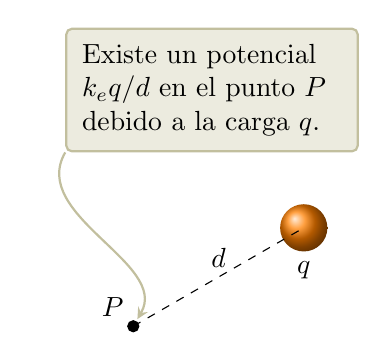
\begin{tikzpicture}[>=stealth]
    \coordinate (P) at (0,0);
    \shade[ball color=orange] (30:2.5) circle (.3) node[below=3mm] {$q$};
    \draw[dashed] (P) -- node[above] {$d$} (30:2.5);
    \filldraw (P) circle (2pt) node[above left] {$P$};
    \node (cartel) [
      text width=3.3cm,
      align=left,
      fill=yellow!40!black!14,
      draw=yellow!40!black!46,
      thick,
      rounded corners=2pt,
      inner sep=2mm
      ]
      at (1,3) {Existe un potencial $k_e q/d$ en el punto $P$ debido a la carga $q$.};
    \draw[->, thick, color=yellow!40!black!46, shorten >=3pt] 
             (cartel.south west) to[out=240, in=60] (P);
  \end{tikzpicture}
  \caption{Potencial en el punto \(P\) debido a \(q\).}
  \label{fig_potencial_en_un_punto}
\end{marginfigure}


Como se mencionó previamente, la energía potencial \(U\) es relativa a un punto que se ha definido como punto de potencial cero. Esto es importante ya que la definición de potencial eléctrico \(V\) parte del concepto de energía potencial, por cuanto, hereda estos comportamientos. Esto implica que si usted desea conocer el potencial en un punto \(P\) como muestra la figura \ref{fig_potencial_en_un_punto}, entonces primero debe saber cual es el punto de potencial cero\footnote{El potencial en un punto es simplemente un caso especial de la diferencia de potencial, donde el punto de partida (usualmente el infinito para cargas puntuales) tiene un potencial de \qty{0}{\volt}.}. De este modo, la distancia de \(P\) a dicho punto de potencial cero, dará la diferencia de potencial de \(P\) con respecto al punto de potencial cero, y consecuentemente, el potencial de \(P\). Entonces el potencial \(V\) en el punto \(P\) es el trabajo requerido para mover la carga de prueba desde el infinito hasta el punto \(P\). Aplicando la definición de potencial, el potencial en el punto \(P\) para una carga puntual se obtiene de la siguiente manera,
\begin{align*}
    V_P &= - \lim_{a \to \infty}\int_{a}^d \vec{E} \cdot d\vec{r}\\
        &= - \lim_{a \to \infty}\int_{a}^d \frac{kq}{r^2} \cdot dr\\
        &= -kq \, \lim_{a \to \infty} \int_{a}^d \frac{1}{r^2} \cdot dr\\
        &= -kq \, \lim_{a \to \infty} \left[ -\frac{1}{r} \right]_{a}^d\\
        &= -kq \, \lim_{a \to \infty} \left[ -\frac{1}{d} + \frac{1}{a} \right]\\
        &= -kq \, \left[ -\frac{1}{d} + 0 \right] \\
    V_P &= k\frac{q}{d} = \lVert\vec{E} (\vec{r})\rVert \, \lVert\vec{r}\rVert \cos(0)
\end{align*}
\marginnote{
  \begin{tcolorbox}[sidenote]
    \footnotesize{Es tentador operar matemáticamente sobre la expresión \eqref{eq:potential_point_charge}, y obtener
    \begin{gather*}
      V_P = k\frac{q}{d} = k\frac{q}{d^2}d \\ 
      \therefore ~ V_P = Ed 
    \end{gather*}
    Y aunque matemáticamente es una tautología, conceptualmente es un error, ya que la carga puntual tiene un campo eléctrico que dependerá de la posición.}
  \end{tcolorbox}
}
siendo \(\lVert \vec{r}\rVert\) el radiovector de módulo \(d\) que apunta a \(P\). Por ser \(\vec{E}\) y \(\vec{r}\) paralelos. Entonces el potencial eléctrico en un punto \(P\) debido a una carga puntual \(q\) es:
\begin{equation}
    \boxed{V_P = k\frac{q}{d}}
    \label{eq:potential_point_charge}
\end{equation}

El potencial eléctrico debido a múltiples cargas puntuales se basa en el principio de superposición, que establece que el potencial eléctrico total en un punto es igual a la suma algebraica de los potenciales individuales producidos por cada carga.
\begin{equation}
    V_\text{total} = \sum_{i=1}^{n} V_i = k \sum_{i=1}^{n} \frac{q_i}{d_i}
\end{equation}

\subsection{Obtención de \texorpdfstring{\(\vec{E}\)}{E} a partir de \texorpdfstring{\(V\)}{V}}

El campo eléctrico \(\vec{E}\) y el potencial eléctrico \(V\) están relacionados, como se muestra en la ecuación \eqref{eq:potential_point_charge}, que se usa para encontrar \(V\) en un punto cuando se conoce \(\vec{E}\). Aunque, también podemos encontrar \(\vec{E}\) a partir de \(V\) usando la relación:
\begin{equation}
  dV = -\vec{E} \cdot d\vec{s}
  \label{eq:field_from_potential_differential}
\end{equation}
y si estamos trabajando con una única coordenada (por ejemplo, un movimiento rectilíneo) podemos escribir la ecuación \eqref{eq:field_from_potential_differential} como:
\[
  dV = -E \, ds \quad \Rightarrow \quad E = -\frac{dV}{ds}
\]

Sin embargo, en general, el potencial eléctrico es una función de las tres coordenadas espaciales. Si \(V(r)\) se da en coordenadas cartesianas, las componentes \((E_x, E_y, E_z)\) del campo eléctrico pueden ser determinadas fácilmente a partir de \(V(x, y, z)\) como derivadas parciales
\begin{equation}
  \boxed{
    \vec{E} = -\nabla V
  }
  \label{eq_gradiente_de_potencial}
\end{equation}
donde \(\nabla\) es el operador nabla, que representa el gradiente del potencial eléctrico. Esta relación indica que el campo eléctrico es igual al negativo del gradiente del potencial eléctrico. En otras palabras, el campo eléctrico apunta en la dirección de mayor disminución del potencial eléctrico.

\begin{tcolorbox}[interesting_data,title=Recordatorio]
El operador nabla \(\nabla\) (u operador del gradiente) es una herramienta matemática usada en cálculo vectorial y análisis multivariable. Se utiliza para representar derivadas en múltiples dimensiones.

Formalmente, el operador nabla se define como:
\[
\nabla = \left( \frac{\partial}{\partial x}, \frac{\partial}{\partial y}, \frac{\partial}{\partial z} \right)
\]
Es un operador vectorial que, aplicado a diferentes tipos de funciones, da lugar a distintos conceptos. En nuestro caso solo vamos a repasar el concepto de gradiente.

Cuando se aplica el operador nabla a una función escalar \( f(x, y, z) \), produce un campo vectorial que apunta en la dirección de mayor incremento de la función. Se expresa como:
\[
\nabla f = \left( \frac{\partial f}{\partial x}, \frac{\partial f}{\partial y}, \frac{\partial f}{\partial z} \right)
\]
Este vector resultante indica la dirección en la que la función crece más rápidamente y su magnitud corresponde a la tasa de cambio máxima. En el caso de \(\vec{E}\) y \(V\), \(\vec{E}\) es el gradiente de \(V\) y por ser \(\vec{E}\) conservativo, \(V\) es su función potencial. Así, \(\nabla V\) representa una función vectorial que apunta en la dirección de mayor disminución del potencial eléctrico, debido al signo negativo, como se indica en la ecuación \eqref{eq_gradiente_de_potencial}.
\end{tcolorbox}

\begin{comment}
  En esta sección se podrían mejorar algunos aspectos.

  Punto número 1: debería demostrar que la fuerza eléctrica (dada por la fuerza de Coulomb) es una fuerza conservativa.

  Punto número 2: debería considerar agregar ejercicios prácticos para aplicar las ecuaciones. Esto puede ser de gran ayuda para un estudiante. Además, en el apartado de la deducción, se podría agregar un ejemplo de un campo considerado como campo vectorial en el espacio, y realizar una demostración de que su rotacional es cero, y el trabajo total es independiente de la trayectoria. Además acompañar esta explicación con esquemas puede ser super intuitivo. Un tornado (con corrientes de viento) genera un campo de velocidades (hay un ejemplo de esto en Khan Academy - buscar: integral de línea en un campo vectorial). \url{https://es.khanacademy.org/math/multivariable-calculus/integrating-multivariable-functions/line-integrals-in-vector-fields-articles/a/line-integrals-in-a-vector-field}

  Un ejemplo interesante podría ser considerar una distribución de cargas puntuales, resolver por definición (Encontrando una expresión del campo eléctrico), y luego demostrar que la fórmula de carga puntual y el principio de superposición se cumplen.

  Ver notas en Serway (p747).
\end{comment}


% \subsection{Capacitores}

\subsubsection{Definición de capacitor}

Un \textbf{capacitor}, también conocido como \textbf{condensador}, es un componente eléctrico pasivo que tiene la capacidad de \textbf{almacenar energía en forma de un campo eléctrico}. Está compuesto por dos conductores (llamados placas) separados por un material dieléctrico, que actúa como aislante.

Cuando se aplica una diferencia de potencial entre las placas, una de ellas acumula carga positiva y la otra carga negativa, generando así un campo eléctrico entre ellas (ver figura \ref{fig:capacitor_charge}). La capacidad del capacitor para almacenar carga depende de sus características físicas y del dieléctrico utilizado.

La capacitancia \( C \) de un capacitor se define como la razón entre la magnitud de la carga almacenada en una de sus placas (\( Q \)) y la diferencia de potencial (\( \Delta V \)) entre las placas:
\begin{equation}
    C = \frac{Q}{V}
    \label{eq:capacitance}    
\end{equation}
donde:
\begin{itemize}
    \item \( C \) es la \textbf{capacitancia} del capacitor, medida en faradios (\(\si{\farad}\)) (siempre es una cantidad positiva).
    \item \( Q \) es la \textbf{carga eléctrica} almacenada en una de las placas del capacitor, medida en coulombs (\(\si{\coulomb}\)).
    \item \( V \) es la \textbf{diferencia de potencial} entre las placas del capacitor, medida en voltios (\(\si{\volt}\)).
\end{itemize}

\begin{figure}[ht]
    \centering
    \includegraphics[width=0.7\textwidth]{capacitor_charge.png}
    \caption{Las cargas negativas fluyen de una placa a la otra.}
    \label{fig:capacitor_charge}
\end{figure}

Un faradio es una unidad muy grande, por lo que en la práctica suelen utilizarse submúltiplos como el microfaradio (\(\mu\si{\farad}\)), nanofaradio (n\(\si{\farad}\)) o picofaradio (p\(\si{\farad}\)).

\paragraph{Premisas y consideraciones importantes:}

La definición \( C = Q/\Delta V \) asume que las placas tienen cargas iguales y opuestas (\( +Q \) y \( -Q \)). Si el capacitor está desbalanceado, la capacitancia no puede calcularse directamente con esta fórmula, pues el sistema ya no es un capacitor ideal.

\subsubsection{Geometría de los conductores}

La capacitancia no depende de \(Q\) ni de \(\Delta V\), sino de la geometría del capacitor y del material dieléctrico entre sus placas.

\paragraph{1. Capacitor de placas planas paralelas}

Por ejemplo si se tienen \hl{placas paralelas} de depende de factores como el área de las placas (\(A\)), la distancia entre ellas (\(d\)) y la permitividad del dieléctrico (\( \varepsilon_0 \) para el vacío) según la siguiente fórmula:

\[
C = \varepsilon_0 \frac{A}{d}
\]

donde:
\begin{itemize}
    \item \( \varepsilon_0 \) es la \textbf{permitividad} del material dieléctrico entre las placas (vacío), que se define como la capacidad de un material para almacenar carga eléctrica en un campo eléctrico. Se mide en faradios por metro (\(\si{\farad\per\meter}\)).
    \item \( A \) es el área de una de las placas del capacitor, medida en metros cuadrados (\(\si{\meter\squared}\)).
    \item \( d \) es la distancia entre las placas, medida en metros (\(\si{\meter}\)).
\end{itemize}

Cuando la \hl{geometría de los conductores} es distinta a la de un capacitor de placas planas y paralelas, la expresión de la capacitancia cambia, aunque el principio físico fundamental sigue siendo el mismo: almacenar energía en forma de campo eléctrico entre conductores separados por un dieléctrico.

\paragraph{2. Capacitor esférico}

Consiste en dos esferas concéntricas de radios \( R_1 \) (interna) y \( R_2 \) (externa). Su capacitancia es:

\[
C = 4\pi \varepsilon_0 \frac{R_1 R_2}{R_2 - R_1}
\]

\paragraph{3. Capacitor cilíndrico}

Está formado por dos cilindros coaxiales, uno de radio interno \( a \) y otro de radio externo \( b \), y de longitud \( L \) (suponiendo \( L \gg b \)). La capacitancia es:

\[
C = \frac{2\pi \varepsilon_0 L}{\ln(b/a)}
\]

\paragraph{4. Geometrías irregulares o generales}

En geometrías más complejas, la capacitancia no puede obtenerse de forma analítica sencilla. En estos casos se recurre a:

\begin{itemize}
    \item Métodos numéricos
    \item Aproximaciones analíticas
    \item Medición experimental
\end{itemize}

Cuando se cambia la geometría, ya no es válida la fórmula simple \( C = \varepsilon_0 \frac{A}{d} \). Es necesario \textbf{considerar la distribución del campo eléctrico} que surge de la nueva disposición geométrica, y calcular la capacitancia a partir de las definiciones fundamentales, como:

\[
C = \frac{Q}{V}
\]
donde \( V \) ahora debe calcularse usando la ley de Gauss o integrando el campo eléctrico apropiado para la geometría dada.

\subsubsection{Energía almacenada en un capacitor}

La fórmula de la energía almacenada en un capacitor,

\begin{equation}
    U = \frac{1}{2} QV
\end{equation}
puede demostrarse considerando el trabajo necesario para cargar el capacitor, es decir, para mover carga desde una placa a la otra en contra del campo eléctrico generado.

\paragraph{Demostración}

Supongamos que inicialmente el capacitor no tiene carga. Para cargarlo, se debe transferir carga desde una placa hacia la otra (esto lo realizará una batería). En un instante cualquiera, si la carga acumulada es \( q \), la diferencia de potencial entre las placas es:

\[
V(q) = \frac{q}{C}
\]

Para mover una carga diferencial \( dq \) contra esta diferencia de potencial, se debe realizar un trabajo diferencial:

\[
dW = V(q) \, dq = \frac{q}{C} \, dq
\]


Entonces, el trabajo total \( W \) para cargar el capacitor desde \( q = 0 \) hasta \( q = Q \) es:

\[
W = \int_{0}^{Q} \frac{q}{C} \, dq = \frac{1}{C} \int_{0}^{Q} q \, dq = \frac{1}{C} \cdot \frac{Q^2}{2} = \frac{1}{2} \frac{Q^2}{C}
\]

Ese trabajo realizado es la energía almacenada en el campo eléctrico del capacitor, por lo tanto:

\[
U = \frac{1}{2} \frac{Q^2}{C}
\]

Como \( Q = CV \), podemos reemplazar en la expresión para obtener las otras formas equivalentes de la energía:

- En función de \( Q \) y \( V \):

\[
U = \frac{1}{2} QV
\]

- En función de \( C \) y \( V \):

\[
U = \frac{1}{2} CV^2
\]

Estas tres expresiones son equivalentes, y se utilizan según las variables conocidas en un problema.

\textbf{Interpretación física:} La energía \( U \) no está en la carga como tal, sino en el campo eléctrico que se establece entre las placas del capacitor. Esta energía puede recuperarse, por ejemplo, al descargar el capacitor en un circuito.

\subsubsection{Dieléctrico en un capacitor}

El dieléctrico es un material aislante que se coloca entre las placas de un capacitor. Su función principal es modificar el campo eléctrico dentro del capacitor y, como consecuencia, aumentar su capacitancia sin necesidad de cambiar su geometría.

\paragraph{¿Qué hace un dieléctrico?}

\begin{figure}[ht]
    \centering
    \includegraphics[width=0.8\textwidth]{capacitor_dielectric.png}
    \caption{Polarización de un dieléctrico en un capacitor.}
    \label{fig:capacitor_dieletrico}
\end{figure}
Cuando se introduce un dieléctrico entre las placas de un capacitor:
\begin{enumerate}
    \item Se polariza: Las moléculas del dieléctrico se alinean parcialmente con el campo eléctrico, creando campos eléctricos internos opuestos al campo aplicado.
    \item Reduce el campo eléctrico efectivo entre las placas.
    \item Esto implica que, para una misma cantidad de carga \( Q \), la diferencia de potencial \( V \) disminuye.
    \item Como \( C = \frac{Q}{V} \), una menor \( V \) implica una mayor capacitancia.
\end{enumerate}
\newpage
\paragraph{Permitividad relativa \( \varepsilon_r \)}

El efecto del dieléctrico se caracteriza mediante una constante adimensional llamada permitividad relativa o constante dieléctrica, denotada por:

\[
\varepsilon_r = \frac{\varepsilon}{\varepsilon_0}
\]

\begin{itemize}
    \item \( \varepsilon_r \) es la permitividad relativa del material dieléctrico.
    \item \( \varepsilon \) es la permitividad del material dieléctrico.
\end{itemize}

Algunas bibliografias utilizan la letra ``k'' cursiva (\textit{k}) para referirse a la constante dieléctrica, aunque usar \( \varepsilon_r \) evita confusión con la constante \(k\) d\textsl{}e la ley de Coulomb.

Cuando se introduce un dieléctrico completamente entre las placas, la capacitancia del capacitor se modifica de:

\[
C_0 = \varepsilon_0 \frac{A}{d}
\quad \text{(sin dieléctrico)}
\]

a:

\[
C = \varepsilon_0 \varepsilon_r \frac{A}{d} = \varepsilon \frac{A}{d}
\quad \text{(con dieléctrico)}
\]

Por lo tanto:

\begin{equation}
    \boxed{C = \varepsilon_r C_0}
    \label{eq:capacitance_dielectric}
\end{equation}

Esto significa que la capacitancia aumenta en un factor \( \varepsilon_r \), que típicamente está entre 2 y 10 para muchos materiales comunes, aunque puede ser mucho mayor en materiales especiales.

\paragraph{Energía almacenada con dieléctrico}

La energía también cambia dependiendo de cómo se conecta el capacitor:

\textbf{Caso 1: } el capacitor está desconectado de la fuente y se inserta el dieléctrico:
\begin{itemize}
    \item \( Q \) se mantiene constante (esta desconectado de la fuente).
    \item \( V \) disminuye (por el campo opuesto del dielectrico).
    \item \( C \) aumenta.
    \item La energía disminuye: parte de la energía se transfiere al dieléctrico como trabajo de polarización.
\end{itemize}

\[
U = \frac{1}{2} \frac{Q^2}{C} \quad \text{(disminuye porque } C \text{ aumenta)}
\]

\textbf{Caso 2: } el capacitor está conectado a una fuente constante \( V \) al insertar el dieléctrico:
\begin{itemize}
    \item \( V \) se mantiene constante.
    \item \( Q \) aumenta (la fuente compensa la disminución de \( V \)).
    \item \( C \) aumenta.
    \item La energía almacenada aumenta, y esta energía adicional proviene de la fuente de voltaje.
\end{itemize}

\[
U = \frac{1}{2} C V^2 \quad \text{(aumenta porque } C \text{ aumenta)}
\]

\paragraph{Resumen de efectos del dieléctrico}

El dieléctrico tiene varios efectos importantes en un capacitor:
\begin{itemize}
    \item Aumenta la capacitancia (\( C \)).
    \item Reduce el campo eléctrico (\( E \)) entre las placas.
    \item Almacena energía adicional en forma de polarización.
    \item Modifica la energía almacenada (\( U \)).
    \item Cambia la expresión de capacitancia (\( C \)) dependiendo de si el capacitor está conectado a una fuente o no.
\end{itemize}

\subsubsection{Potencial o Voltaje de ruptura de un dieléctrico}

El voltaje de ruptura (también llamado tensión de ruptura o dieléctrica) es la máxima diferencia de potencial que puede aplicarse entre las placas de un capacitor (o entre dos puntos de un aislante) antes de que el material dieléctrico falle y se vuelva conductor.

\paragraph{¿Qué ocurre cuando se supera el voltaje de ruptura?}

Cuando el campo eléctrico en el dieléctrico supera un valor crítico, llamado intensidad de campo de ruptura (o rigidez dieléctrica), el material se ioniza, es decir, sus átomos o moléculas pierden electrones debido al campo intenso, y se produce una descarga eléctrica: el dieléctrico pierde su capacidad aislante y permite el paso de corriente.

Esto puede generar:

\begin{itemize}
    \item Chispas o arcos eléctricos.
    \item Daño permanente al capacitor.
    \item Cortocircuitos en circuitos eléctricos.
\end{itemize}

\paragraph{Campo eléctrico de ruptura \( E_{\text{ruptura}} \)}

Se expresa como:

\[
E_{\text{ruptura}} = \frac{V_{\text{ruptura}}}{d}
\]
donde:
\begin{itemize}
    \item \( V_{\text{ruptura}} \) es el voltaje de ruptura.
    \item \( d \) es la distancia entre las placas del capacitor.
    \item \( E_{\text{ruptura}} \) es la intensidad de campo eléctrico de ruptura, medida en voltios por metro (V/m) o más comúnmente en megavoltios por metro (MV/m).
\end{itemize}

\subparagraph{Valores típicos de \( V_{\text{ruptura}} \)}

\begin{table*}[ht]
    \centering
    \begin{tabular}{|c|c|c|}
        \hline
        \textbf{Material} & \textbf{Constante dieléctica \(\varepsilon_r\)} & \textbf{Resistencia}\\ 
        &&\textbf{de ruptura (MV/m)} \\
        \hline
        Aire & 1.00059 & 3 \\
        Papel impregnado & 3.5 & 11 \\
        Nylon & 3.4 & 14 \\
        Polietileno & 2.56 & 24 \\
        Teflón & 2.1 & 60 \\
        \hline
    \end{tabular}
    \caption{Valores típicos de tensión de ruptura para diferentes dieléctricos.}
    \label{tab:ruptura}
\end{table*}

\subsubsection{Capacitores en serie y paralelo}

Los capacitores pueden conectarse en serie o en paralelo, y la forma en que se conectan afecta la capacitancia total del circuito.

\paragraph{1. Capacitores en paralelo}

\begin{figure}[ht]
    \centering
    \includegraphics[width=0.8\textwidth]{capacitors_parallel.png}
    \caption{Configuración de capacitores en paralelo.}
    \label{fig:capacitors_parallel}    
\end{figure}

\textbf{Configuración:} Todos los capacitores están conectados a la misma diferencia de potencial \( V \). Es decir:

\[
V_1 = V_2 = \dots = V_n = V
\]

\textbf{Carga total:} La carga total almacenada es la suma de las cargas individuales:

\[
Q_{\text{total}} = Q_1 + Q_2 + \dots + Q_n
\]

Como \( Q_i = C_i V \), entonces:

\[
Q_{\text{total}} = C_1 V + C_2 V + \dots + C_n V = \left( C_1 + C_2 + \dots + C_n \right) V
\]

Pero, por definición:

\[
Q_{\text{total}} = C_{\text{eq}} V
\]

Comparando ambas expresiones:

\[
C_{\text{eq}} = C_1 + C_2 + \dots + C_n
\]

\textbf{Resultado:} La capacitancia equivalente en paralelo es la suma directa de las capacitancias individuales.

Cuando los capacitores están conectados en paralelo, la capacitancia total \( C_{\text{total}} \) se calcula sumando las capacitancias individuales:
\begin{equation}
    \boxed{C_{\text{total}} = C_1 + C_2 + C_3 + \ldots}
    \label{eq:capacitance_parallel}
\end{equation}
donde \( C_1, C_2, C_3, \ldots \) son las capacitancias individuales de los capacitores conectados en paralelo.

\paragraph{2. Capacitores en serie}

\begin{figure}[ht]
    \centering
    \includegraphics[width=0.9\textwidth]{capacitors_series.png}
    \caption{Configuración de capacitores en serie.}
    \label{fig:capacitors_series}
\end{figure}

\textbf{Configuración:} Todos los capacitores están conectados uno tras otro, por lo tanto, la misma carga \( Q \) pasa por todos. Es decir:

\[
Q_1 = Q_2 = \dots = Q_n = Q
\]

¿Por qué? Porque la carga del capacitor más pequeño actua como ``cuello de botella'' resultando en que la carga total es la misma en todos los capacitores.
\begin{figure}[ht]
    \centering
    \includegraphics[width=0.9\textwidth]{capacitor_series_charge.png}
    \caption{La carga en ambos capacitores es la misma.}
    \label{fig:capacitors_series_charge}
\end{figure}

Como se puede ver en la figura \ref{fig:capacitors_series_charge}, la carga en ambos capacitores es la misma porque el capacitor \(C_2\) (más pequeño) está completamente cargado, esto provoca que el capacitor \(C_1\) (más grande) se vea limitado y no se use toda la capacidad. Esto es así porque los electrones se mueven de la placa izquierda del capacitor \(C_1\) a la placa derecha del capacitor \(C_2\). Cuando el capacitor \(C_2\) se carga completamente no puede acumular más carga. Por otro lado el capacitor \(C_1\) aún tiene electrones en su placa izquierda, pero estos electrones no tienen a donde ir, por lo que no se puede acumular más carga. Lo mismo sucede en las placas del medio de ambos capacitores. En una configuración en serie, la carga del capacitor más pequeño será la carga total usada de la batería.

Como la carga en todos los capacitores es la misma, la diferencia de potencial entre las placas de cada capacitor será diferente. La diferencia de potencial total es la suma de las diferencias de potencial individuales:

\[
V_{\text{total}} = V_1 + V_2 + \dots + V_n
\]

Pero \( V_i = \frac{Q}{C_i} \), entonces:

\[
V_{\text{total}} = \frac{Q}{C_1} + \frac{Q}{C_2} + \dots + \frac{Q}{C_n} = Q \left( \frac{1}{C_1} + \frac{1}{C_2} + \dots + \frac{1}{C_n} \right)
\]

Por definición, \( V_{\text{total}} = \frac{Q}{C_{\text{eq}}} \), así que:

\[
\frac{Q}{C_{\text{eq}}} = Q \left( \frac{1}{C_1} + \frac{1}{C_2} + \dots + \frac{1}{C_n} \right)
\]

Dividiendo ambos lados por \( Q \neq 0 \):

\[
\frac{1}{C_{\text{eq}}} = \frac{1}{C_1} + \frac{1}{C_2} + \dots + \frac{1}{C_n}
\]

\textbf{Resultado:} La inversa de la capacitancia equivalente en serie es igual a la suma de las inversas de las capacitancias individuales.

\begin{equation}
    \boxed{\frac{1}{C_{\text{total}}} = \frac{1}{C_1} + \frac{1}{C_2} + \frac{1}{C_3} + \ldots}
    \label{eq:capacitance_series}
\end{equation}
donde \( C_1, C_2, C_3, \ldots \) son las capacitancias individuales de los capacitores conectados en serie.

% \begin{table}[h]
    \centering
    \renewcommand{\arraystretch}{1.5}
    \begin{tabular}{|>{\bfseries}l|l|}
        \hline
        \textbf{Concepto} & \textbf{Definición Matemática y Explicación} \\ \hline
        
        \textbf{Ley de Coulomb} & 
        $\vec{F} = k \frac{q_1 q_2}{r^2} \hat{r}$ \\
        & Fuerza entre dos cargas puntuales ($q_1$, $q_2$): \\
        & - $k = \frac{1}{4\pi\varepsilon_0}$ (Constante de Coulomb) \\
        & - $r$: Distancia entre cargas, $\hat{r}$: Vector unitario radial. \\ \hline
        
        \textbf{Campo Eléctrico} & 
        $\vec{E} = \frac{\vec{F}}{q_0} = k \frac{Q}{r^2} \hat{r}$ \\
        & Fuerza por unidad de carga ($q_0$) en un punto: \\
        & - Dirección: Radial para cargas puntuales. \\ \hline
        
        \textbf{Flujo Eléctrico} & 
        $\Phi_E = \int_S \vec{E} \cdot d\vec{A}$ \\
        & Medida del "número de líneas de campo" que atraviesan \\
        & una superficie $S$: \\
        & - $d\vec{A}$: Vector área (normal a la superficie). \\ \hline
        
        \textbf{Ley de Gauss} & 
        $\oint \vec{E} \cdot d\vec{A} = \frac{Q_{\text{int}}}{\varepsilon_0}$ \\
        & Relación entre flujo eléctrico a través de una superficie \\
        & cerrada y la carga encerrada ($Q_{\text{int}}$). \\ \hline
        
        \textbf{Energía Potencial} & 
        $U = k \frac{q_1 q_2}{r}$ \\
        & Trabajo para reunir cargas desde el infinito: \\
        & - $U > 0$ (repulsión), $U < 0$ (atracción). \\ \hline
        
        \textbf{Trabajo Eléctrico} & 
        $W = -\Delta U = q \Delta V$ \\
        & Trabajo realizado por el campo para mover una carga $q$: \\
        & - Depende de la diferencia de potencial ($\Delta V$). \\ \hline
        
        \textbf{Potencial Eléctrico} & 
        $V = \frac{U}{q_0} = k \frac{Q}{r}$ \\
        & Energía potencial por unidad de carga ($q_0$): \\
        & - Escalar, medido en voltios (V). \\ \hline
    \end{tabular}
    \caption{Resumen de conceptos fundamentales de Electroestática.}
    \label{tab:electrostatica}
\end{table}
